\documentclass{article}
\usepackage[paperwidth=33cm,paperheight=7.5cm,margin=0cm]{geometry}
\usepackage[utf8]{inputenc}
\usepackage[T1]{fontenc}
\usepackage{lmodern}
\usepackage{tikz}
\usetikzlibrary{shapes.geometric, positioning, arrows.meta, fit, backgrounds, calc}

\pagestyle{empty}

\begin{document}
\centering
\vspace*{\fill}
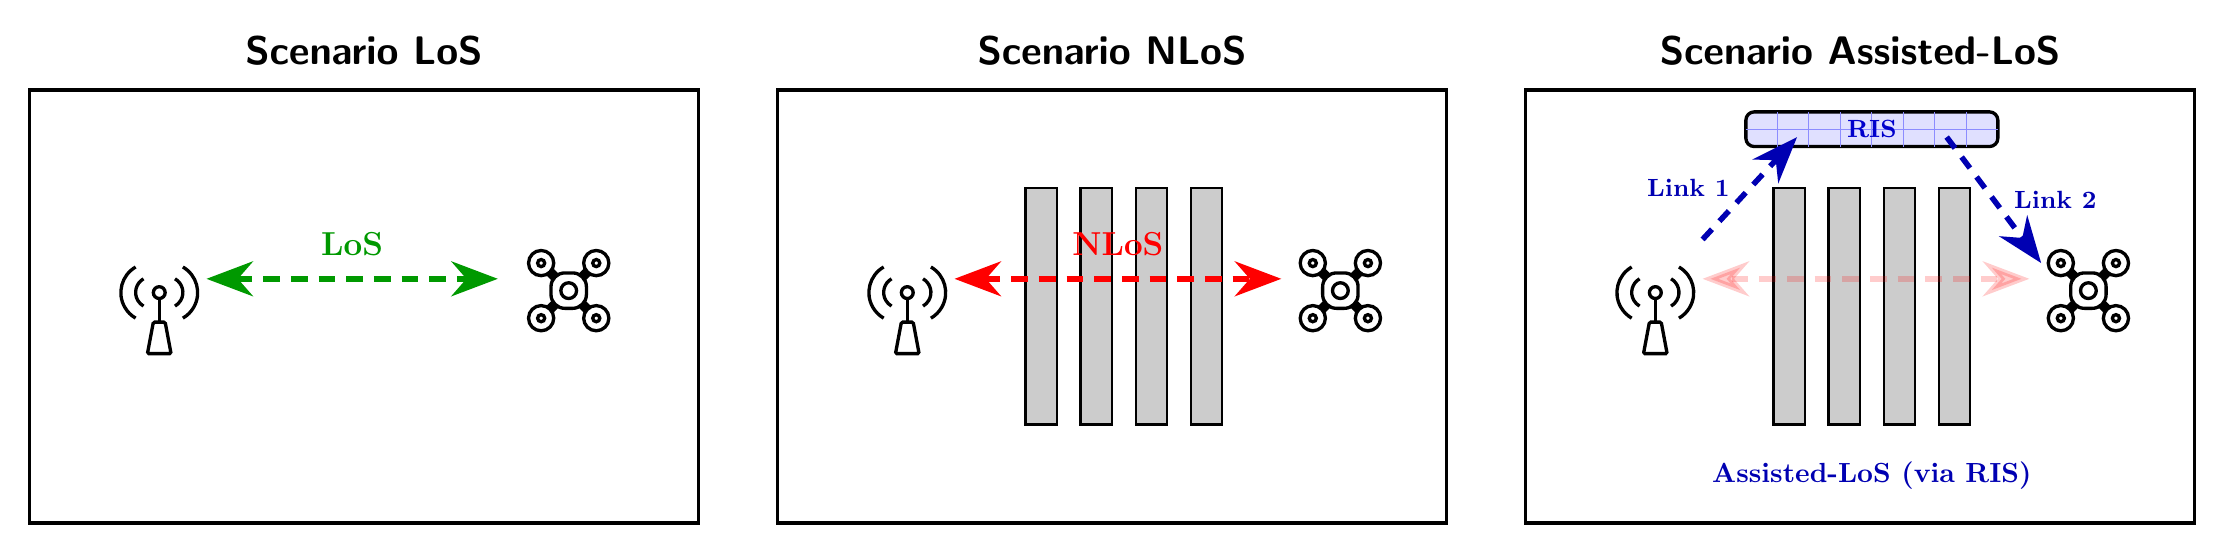
\begin{tikzpicture}[
    font=\sffamily,
    warehouse_walls/.style={
        draw=black, very thick,
        minimum width=8.5cm, minimum height=5.5cm,
        fill=white, inner sep=0pt
    },
    shelf/.style={
        draw=black, fill=gray!40, thick,
        minimum width=0.4cm, minimum height=3cm
    },
    los_line/.style={
        {Stealth[scale=1.4]}-{Stealth[scale=1.4]},
        green!60!black, line width=2pt,
        dashed, dash pattern=on 6pt off 4pt
    },
    nlos_line/.style={
        {Stealth[scale=1.4]}-{Stealth[scale=1.4]},
        red, line width=2pt,
        dashed, dash pattern=on 6pt off 4pt
    },
    alos_line/.style={
        -{Stealth[scale=1.4]},
        blue!70!black, line width=2pt,
        dashed, dash pattern=on 5pt off 4pt
    }
]

%% ── BS Symbol ──────────────────────────────
\tikzset{bs/.pic={
    \begin{scope}[scale=0.50]
    \draw[very thick, fill=white, rounded corners=0.5pt]
        (-0.3,0)--(0.3,0)--(0.15,0.8)--(-0.15,0.8)--cycle;
    \draw[very thick](0,0.8)--(0,1.4);
    \draw[very thick, fill=white](0,1.55) circle(0.15);
    \draw[very thick](0.4,1.9)  arc(60:-60:0.40);
    \draw[very thick](0.6,2.2)  arc(60:-60:0.75);
    \draw[very thick](-0.4,1.9) arc(120:240:0.40);
    \draw[very thick](-0.6,2.2) arc(120:240:0.75);
    \end{scope}
}}

%% ── Drone Symbol ───────────────────────────
\tikzset{drone/.pic={
    \begin{scope}[scale=0.50]
    \draw[line width=3.5pt](-0.7,-0.7)--(0.7,0.7);
    \draw[line width=3.5pt](-0.7,0.7)--(0.7,-0.7);
    \draw[very thick, fill=white, rounded corners=5pt]
        (-0.45,-0.45) rectangle (0.45,0.45);
    \draw[very thick, fill=white](0,0) circle(0.20);
    \foreach \x/\y in {-0.7/-0.7, 0.7/0.7, -0.7/0.7, 0.7/-0.7}{
        \draw[very thick, fill=white](\x,\y) circle(0.32);
        \draw[very thick, fill=white](\x,\y) circle(0.09);
    }
    \end{scope}
}}

%% ── RIS Symbol – ORIZZONTALE (pannello piatto) ─
\tikzset{ris_h/.pic={
    \begin{scope}
    % pannello orizzontale
    \draw[very thick, fill=blue!12, rounded corners=3pt]
        (-1.6,-0.22) rectangle (1.6,0.22);
    % linee verticali (elementi)
    \foreach \x in {-1.2,-0.8,-0.4,0.0,0.4,0.8,1.2}{
        \draw[blue!45, thin](\x,-0.22)--(\x,0.22);
    }
    % linea orizzontale centrale
    \draw[blue!45, thin](-1.6,0)--(1.6,0);
    % etichetta
    \node[font=\small\bfseries, text=blue!80!black] at (0,0) {RIS};
    \end{scope}
}}

% ══════════════════════════════════════
%  PANNELLO 1 – LoS
% ══════════════════════════════════════
\begin{scope}[shift={(0,0)}]
    \node[warehouse_walls] (w1) at (0,0) {};
    \node[anchor=south, yshift=5pt] at (w1.north)
        {\textbf{\Large Scenario LoS}};

    \pic at (-2.6,-0.6) {bs};
    \pic at ( 2.6, 0.2) {drone};

    \draw[los_line] (-2.0,0.35) -- (1.7,0.35)
        node[midway,above=4pt,font=\bfseries\large\color{green!60!black}]{LoS};
\end{scope}

% ══════════════════════════════════════
%  PANNELLO 2 – NLoS
% ══════════════════════════════════════
\begin{scope}[shift={(9.5,0)}]
    \node[warehouse_walls] (w2) at (0,0) {};
    \node[anchor=south, yshift=5pt] at (w2.north)
        {\textbf{\Large Scenario NLoS}};

    \pic at (-2.6,-0.6) {bs};

    \foreach \x in {-0.9,-0.2,0.5,1.2}{
        \node[shelf] at (\x,0) {};
    }

    \pic at (2.9, 0.2) {drone};

    \draw[nlos_line] (-2.0,0.35) -- (2.15,0.35)
        node[midway,above=4pt,font=\bfseries\large\color{red}]{NLoS};
\end{scope}

% ══════════════════════════════════════
%  PANNELLO 3 – Assisted-LoS
% ══════════════════════════════════════
\begin{scope}[shift={(19,0)}]
    \node[warehouse_walls] (w3) at (0,0) {};
    \node[anchor=south, yshift=5pt] at (w3.north)
        {\textbf{\Large Scenario Assisted-LoS}};

    % Base Station (sinistra)
    \pic at (-2.6,-0.6) {bs};

    % Scaffalature (bloccano path diretto)
    \foreach \x in {-0.9,-0.2,0.5,1.2}{
        \node[shelf] at (\x,0) {};
    }

    % Drone (destra, oltre le scaffalature)
    \pic at (2.9, 0.2) {drone};

    % RIS ORIZZONTALE – montata in alto (soffitto), centrata
    \pic at (0.15, 2.25) {ris_h};

    % Percorso diretto bloccato (sbiadito)
    \draw[nlos_line, opacity=0.20] (-2.0,0.35) -- (2.15,0.35);

    % Link 1: BS → RIS (sale in diagonale a sinistra fino alla RIS)
    \draw[alos_line] (-2.0, 0.85) -- (-0.80, 2.15)
        node[midway, left=3pt, font=\small\bfseries\color{blue!70!black}]
        {Link 1};

    % Link 2: RIS → Drone (scende a destra dalla RIS al drone)
    \draw[alos_line] (1.10, 2.15) -- (2.30, 0.55)
        node[midway, right=3pt, font=\small\bfseries\color{blue!70!black}]
        {Link 2};

    % Annotazione in basso
    \node[font=\normalsize\bfseries\color{blue!70!black}]
        at (0.15,-2.15) {Assisted-LoS (via RIS)};
\end{scope}

\end{tikzpicture}
\vspace*{\fill}
\end{document}
